\section{Problem 1}
\subsection{Technics}

    \begin{frame}
        \frametitle{Using Eigen Library for C++}

        \begin{itemize}
            \item Compute eigenvalues using EigenSolver.
            \item Compute \(d_i\) and \(j_i\).
            \item Construct the Jordan block for Jordan Canonical From
        \end{itemize}

    \end{frame}

    \subsection{Results}
    \begin{frame}
        \frametitle{Program Result}
        % \framesubtitle{子标题}
        
        \begin{figure}
            \centering
            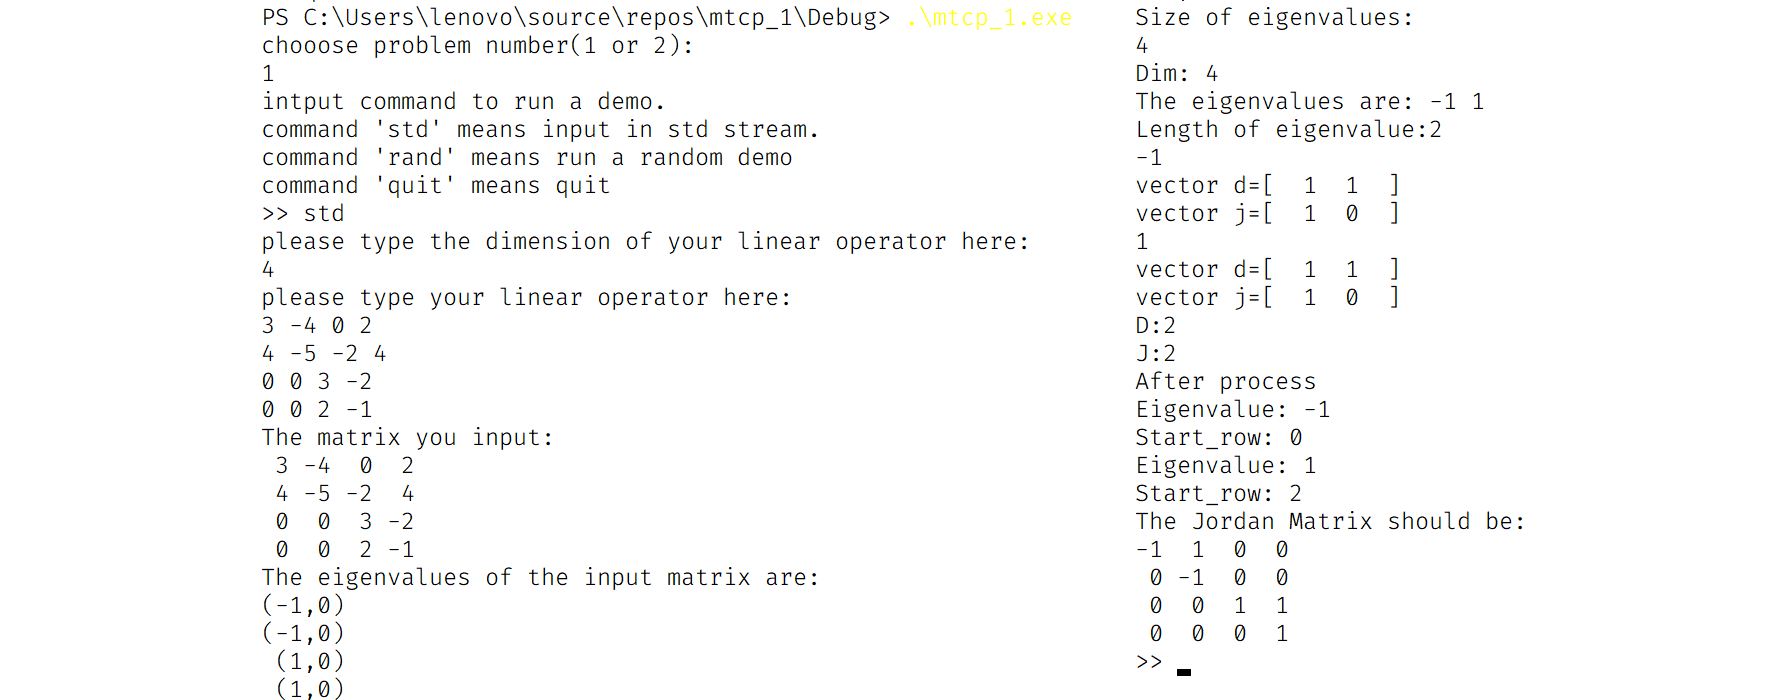
\includegraphics[height = 0.65\textheight]{img/result1.png}
            \caption{demo: input from user-defined matrix}
        \end{figure}
        
    \end{frame}